%!TEX program = xelatex
%!TEX spellcheck = en_GB
\documentclass[final]{article}
% Include all project wide packages here.
%\usepackage{fullpage}
\usepackage[a4paper,margin=2.5cm,top=2cm]{geometry}
\usepackage{polyglossia}
\setmainlanguage{english}
\usepackage{csquotes}
\usepackage{graphicx}
\usepackage{pdfpages}
\usepackage{caption}
\usepackage[list=true]{subcaption}
\usepackage{float}
\usepackage{standalone}
\usepackage{import}
\usepackage{tocloft}
\usepackage{wrapfig}
\usepackage{authblk}
\usepackage{array}
\usepackage{booktabs}
\usepackage[title,titletoc]{appendix}
\usepackage{fontspec}
\usepackage{pgfplots}
\usepackage{tikz}
\usepackage[binary-units=true,table-auto-round]{siunitx}
\usepackage{units}
\usepackage{amsmath}
\usepackage{mathtools}
\usepackage{unicode-math}
\usepackage{rotating}
\usepackage{titlesec}
\usepackage{titletoc}
\usepackage{blindtext}
\usepackage{color}
\usepackage{enumitem}
\usepackage{tabularx}
\usepackage{titling}
\usepackage{multirow}
\usepackage[%
siunitx,
fulldiodes,
europeanvoltages,
europeancurrents,
europeanresistors,
americaninductors,
smartlabels]{circuitikz}

\newcommand{\matlab}{{\textsc{matlab }}}

\usetikzlibrary{calc}
\usetikzlibrary{positioning}
\usetikzlibrary{automata}
\usetikzlibrary{arrows.meta}

\tikzstyle{every state}=[fill=tu-cyan,align=center,draw=black,line width=1pt,node distance=3cm,minimum width = 1.8cm]%for FSMs casper
\tikzstyle{every initial by arrow}=[initial text={Reset}]
\newcommand{\setpathasarrows}{\tikzstyle{every path}=[auto,line width=1.5pt,line cap=round,line join=round]}

\pgfplotsset{compat=newest}
\pgfplotsset{plot coordinates/math parser=false}
\usetikzlibrary{plotmarks}
\usepgfplotslibrary{patchplots}
\newlength\figureheight
\newlength\figurewidth

\tikzset{every axis/.style={xticklabel style={align=right}}}

\usepackage[
%backend=bibtex,
backend=biber,
	texencoding=utf8,
    bibencoding=utf8,
    style=numeric,
    citestyle=numeric,
    sortlocale=en_US,
    language=auto,
    backref=true,
    abbreviate=false,
    date=edtf,
    seconds=true
]{biblatex}

\usepackage{listings}
\newcommand{\includecode}[4][c]{\lstinputlisting[caption=#2, escapechar=, style=#1,label=#4]{#3}}
\newcommand{\superscript}[1]{\ensuremath{^{\textrm{#1}}}}
\newcommand{\subscript}[1]{\ensuremath{_{\textrm{#1}}}}


\newcommand{\chapternumber}{\thechapter}
\renewcommand{\appendixname}{Appendix}
\renewcommand{\appendixtocname}{Appendices}
\renewcommand{\appendixpagename}{Appendices}


\setlist[enumerate]{labelsep=*, leftmargin=1.5pc}
\setlist[enumerate,1]{label=\arabic*., ref=\arabic*}
\setlist[enumerate,2]{label=\arabic*.,ref=\theenumi.\arabic*}
\setlist[enumerate,3]{label=\arabic*., ref=\theenumii.\arabic*}

%\setcounter{chapter}{-1} %start chapter numbers with 0

\usepackage{xr-hyper}
\usepackage[hidelinks]{hyperref} %<--------ALTIJD ALS LAATSTE
\usepackage[nameinlink,noabbrev,capitalise]{cleveref} %<------- Clever Ref moet na hyperref
\crefname{app}{Appendix}{Appendices}
%\renewcommand{\familydefault}{\sfdefault}


\setmainfont{Myriad Pro}[Ligatures={Common,TeX}]
%\setmathfont{Asana Math}
\setmathfont{Asana-Math.otf}
\setmonofont[Scale=0.9]{Lucida Console}
\newfontfamily\headingfont{Minion Pro}[Ligatures={Common,TeX}]


%Design colors
\definecolor{accent1}{RGB}{0,100,200}
\definecolor{accent2}{RGB}{0,50,100}
\definecolor{tu-cyan}{RGB}{0,166,214}

\newcommand{\hsp}{\hspace{20pt}}
% \titleformat{\chapter}[hang]{\Huge\headingfont}{\chapternumber\hsp\textcolor{accent2}{|}\hsp}{0pt}{\Huge\headingfont}

% \titleformat{name=\chapter,numberless}[hang]{\Huge\headingfont}{\hsp\textcolor{accent2}{|}\hsp}{0pt}{\Huge\headingfont}

% \titleformat{\section}[block]{\LARGE\headingfont}{\arabic{chapter}.\arabic{section}}{0.4em}{}
% \titleformat{\subsection}[block]{\Large\headingfont}{\arabic{chapter}.\arabic{section}.\arabic{subsection}}{0.4em}{}
% \titleformat{\subsubsection}[block]{\large\headingfont}{\arabic{chapter}.\arabic{section}.\arabic{subsection}.\arabic{subsubsection}}{0.4em}{}
\renewcommand{\arraystretch}{1.2}
\renewcommand{\baselinestretch}{1.25} 

\renewcommand\cfttoctitlefont{\headingfont\Huge}
\renewcommand\cftloftitlefont{\headingfont\Huge}
\renewcommand\cftlottitlefont{\headingfont\Huge}
\setcounter{lofdepth}{2}
\setcounter{lotdepth}{2}


\setlength{\parindent}{0pt}
\setlength{\parskip}{1em}

\captionsetup{width=0.9\textwidth}

%SIuntix settings:
%default: 0V to 10V
%custom: 0 - 10V
\sisetup{range-phrase=--}
\sisetup{range-units=single}
\DeclareSIUnit\years{years}

%For code listings
\definecolor{black}{rgb}{0,0,0}
\definecolor{browntags}{rgb}{0.65,0.1,0.1}
\definecolor{bluestrings}{rgb}{0,0,1}
\definecolor{graycomments}{rgb}{0.4,0.4,0.4}
\definecolor{redkeywords}{rgb}{1,0,0}
\definecolor{bluekeywords}{rgb}{0.13,0.13,0.8}
\definecolor{greencomments}{rgb}{0,0.5,0}
\definecolor{redstrings}{rgb}{0.9,0,0}
\definecolor{purpleidentifiers}{rgb}{0.01,0,0.01}


\lstdefinestyle{csharp}{
language=[Sharp]C,
showspaces=false,
showtabs=false,
breaklines=true,
showstringspaces=false,
breakatwhitespace=true,
escapeinside={(*@}{@*)},
columns=fullflexible,
commentstyle=\color{greencomments},
keywordstyle=\color{bluekeywords}\bfseries,
stringstyle=\color{redstrings},
identifierstyle=\color{purpleidentifiers},
basicstyle=\ttfamily\small}

\lstdefinestyle{c}{
language=C,
showspaces=false,
showtabs=false,
breaklines=true,
showstringspaces=false,
breakatwhitespace=true,
escapeinside={(*@}{@*)},
columns=fullflexible,
commentstyle=\color{greencomments},
keywordstyle=\color{bluekeywords}\bfseries,
stringstyle=\color{redstrings},
identifierstyle=\color{purpleidentifiers},
}

\lstdefinestyle{matlab}{
language=Matlab,
showspaces=false,
showtabs=false,
breaklines=true,
showstringspaces=false,
breakatwhitespace=true,
escapeinside={(*@}{@*)},
columns=fullflexible,
commentstyle=\color{greencomments},
keywordstyle=\color{bluekeywords}\bfseries,
stringstyle=\color{redstrings},
identifierstyle=\color{purpleidentifiers}
}

\lstdefinestyle{vhdl}{
language=VHDL,
showspaces=false,
showtabs=false,
breaklines=true,
showstringspaces=false,
breakatwhitespace=true,
escapeinside={(*@}{@*)},
columns=fullflexible,
commentstyle=\color{greencomments},
keywordstyle=\color{bluekeywords}\bfseries,
stringstyle=\color{redstrings},
identifierstyle=\color{purpleidentifiers}
}

\lstdefinestyle{xaml}{
language=XML,
showspaces=false,
showtabs=false,
breaklines=true,
showstringspaces=false,
breakatwhitespace=true,
escapeinside={(*@}{@*)},
columns=fullflexible,
commentstyle=\color{greencomments},
keywordstyle=\color{redkeywords},
stringstyle=\color{bluestrings},
tagstyle=\color{browntags},
morestring=[b]",
  morecomment=[s]{<?}{?>},
  morekeywords={xmlns,version,typex:AsyncRecords,x:Arguments,x:Boolean,x:Byte,x:Char,x:Class,x:ClassAttributes,x:ClassModifier,x:Code,x:ConnectionId,x:Decimal,x:Double,x:FactoryMethod,x:FieldModifier,x:Int16,x:Int32,x:Int64,x:Key,x:Members,x:Name,x:Object,x:Property,x:Shared,x:Single,x:String,x:Subclass,x:SynchronousMode,x:TimeSpan,x:TypeArguments,x:Uid,x:Uri,x:XData,Grid.Column,Grid.ColumnSpan,Click,ClipToBounds,Content,DropDownOpened,FontSize,Foreground,Header,Height,HorizontalAlignment,HorizontalContentAlignment,IsCancel,IsDefault,IsEnabled,IsSelected,Margin,MinHeight,MinWidth,Padding,SnapsToDevicePixels,Target,TextWrapping,Title,VerticalAlignment,VerticalContentAlignment,Width,WindowStartupLocation,Binding,Mode,OneWay,xmlns:x}
}

\lstdefinestyle{python}{
language=Python,
showspaces=false,
showtabs=false,
breaklines=true,
showstringspaces=false,
breakatwhitespace=true,
escapeinside={(*@}{@*)},
columns=fullflexible,
commentstyle=\color{greencomments},
keywordstyle=\color{bluekeywords}\bfseries,
stringstyle=\color{redstrings},
identifierstyle=\color{purpleidentifiers},
}

%defaults
\lstset{
basicstyle=\ttfamily\scriptsize ,
extendedchars=false,
numbers=left,
numberstyle=\ttfamily\tiny,
stepnumber=1,
tabsize=4,
numbersep=5pt
}
\addbibresource{../../.library/bibliography.bib}
\begin{document}
\section{Results}
\label{sec:results}
The resulting amount of viable improvements produced with all improvement efforts combined turned out to be three.
The cache was improved in terms of size and part of RAM that could be cached, a new multiplier was designed, and a new divider was designed.
In this section, the impact of the successful improvements on the performance and area footprint of the processor is discussed.

\subsection{Area}
\label{sec:area}
\begin{table}[H]
    \centering
    \caption{Area footprint increase caused by each improvement compared to the original processor implementation}
    \label{tab:areaincrease}
    \begin{tabular}{lllll}
        \toprule
         & \textbf{\SI{8}{\kibi\byte} cache} & \textbf{\SI{16}{\kibi\byte} cache} & \textbf{Multiplier} & \textbf{Divider} \\
        \midrule
        Area ($A_{CLB}$)    &       \num{0}            & \num{5} & \num{535.25}  &   115       \\
        \bottomrule
    \end{tabular}

\end{table}

\Cref{tab:areaincrease} shows the impact of each of the possible processor upgrades on the area footprint.
As discussed in \cref{sec:cache} the \SI{8}{\kibi\byte} does not add any extra area as the original processor was implemented with more room in the cache memory than actually utilised.
The extra area in the \SI{16}{\kibi\byte} design is cause by the addition of four \SI{2}{\kibi\byte} RAM blocks for the cache RAM and one \SI{2}{\kibi\byte} RAM block for the cache tag RAM.
These area increases are rather small compared to the impact of adding a better multiplier and divider.
The multiplier more than doubles the original 514.5 $A_{CLB}$ processor and the divider increases it with 22.4\% due to the extra slices needed for the large amount of adders in both designs.

\subsection{Benchmark cycles}
\begin{table}[H]
    \centering
    \caption{Reduction in amount of benchmark cycles provided by each improvement compared to the original processor}
    \label{tab:cycledecrease}
    \begin{tabular}{lS[table-format=3.3]S[table-format=3.3]S[table-format=3.3]S[table-format=3.3]}
        \toprule
        \textbf{Name}       &  \textbf{\SI{8}{\kibi\byte} cache} & \textbf{\SI{16}{\kibi\byte} cache} & \textbf{Multiplier} & \textbf{Divider} \\
        \midrule
        cjpeg      &  4.787351       & 5.830762   &    0.021205 &     	 0.189012       \\
        divide     &  1.022280       & 9.945005    &   37.822001  &   	 0.101900         \\
        multiply   &  0.385784       & 4.956912   &    23.127938 &    	 0.045826        \\
        pi         &  0.663623       & 3.468797   &    383.919643   &   114.009086                \\
        fir        &  0.891719       & 1.367480   &    102.210450   &  	 0.000000          \\
        rsa        &  13.223744      & 17.353369   &   124.255125    &   0.002088              \\
        ssd        &  37.509906      & 145.664113    & 328.050324      & 2.432114            \\
        ssearch    &  8.820637       & 8.088804   &    0.000053 &     	0.000091           \\
        susan      &  137.363097     & 141.085591   &  517.442442     &  0.658676            \\
        bench\_all &  321.735065     & 454.827757   &  1516.849181     &117.438793                  \\
        \bottomrule
    \end{tabular}
\end{table}


\Cref{tab:cycledecrease} shows the amount of benchmark cycles saved in each improvement with respect to the original implementation.
It can be seen that not each improvement uses the area increase it causes (as seen in \cref{sec:area}) as efficiently as the others.
Different benchmarks benefit from different improvements.
For example, ssearch and cjpeg only seem to gain from increasing the cache size while pi, fir, rsa, susan and ssd really utilise the new divider.
Oddly enough, the only benchmark that sees a significant decrease in benchmark cycles when the divider is implemented is pi while the divide benchmark does not benefit from it at all.

\subsection{Power}
\begin{figure}[H]
\centering
\begin{subfigure}{.5\textwidth}
  \centering
  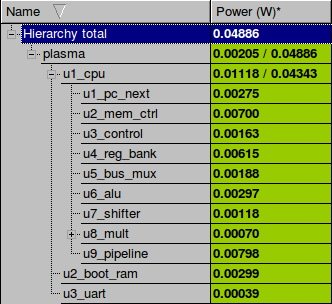
\includegraphics[width=.6\linewidth]{resources/power16mult}
  \caption{\SI{16}{\kibi\byte} + mult (\SI{0.710}{\watt})}
  \label{fig:16multpower}
\end{subfigure}%
\begin{subfigure}{.5\textwidth}
  \centering
  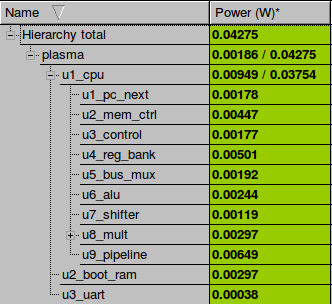
\includegraphics[width=.6\linewidth]{resources/power8multdiv}
  \caption{\SI{8}{\kibi\byte} + mult + div (\SI{0.716}{\watt})}
  \label{fig:8multdivpower}
\end{subfigure}
\begin{subfigure}{.5\textwidth}
  \centering
  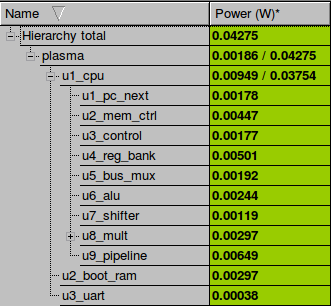
\includegraphics[width=.6\linewidth]{resources/power16multdiv}
  \caption{\SI{16}{\kibi\byte} + mult + div (\SI{0.716}{\watt})}
  \label{fig:16multdivpower}
\end{subfigure}
\caption{Power consumption by hierarchy for three designs with total power estimation between brackets}
\label{fig:powerresults}
\end{figure}

\Cref{fig:powerresults} shows power consumption tables produced by Xilinx ISE for three different designs. Because the power estimation process as laid out by the project manual was a very lengthy process, it was only run for three different designs that looked promising by virtue of their benchmark score and area. As can be expected adding extra components to the design increased the power usage slightly, though the difference with the original \SI{0.698}{\watt} is not that significant. Increasing the cache size from \SI{8}{\kibi\byte} to \SI{16}{\kibi\byte} while keeping the multiplier and the divider in the design did nothing to increase the power usage.

\subsection{Compound metrics}
\label{ssec:compound-metrics}
There are several compound metrics listed below.
\begin{description}

    \item[Benchmark Score] This is in MCyc compensated for a higher running frequency when used, lower is better.
    \item[Performance] This is the reciprocal of the benchmark score, higher is better.
    \item[Perf. per Area] This is the performance times a thousand per area unit ($A_{CLB}$), higher is better.
    \item[BS Area] This is the benchmark score times the area unit divided by a million.
    \item[Perf. per watt] This is the performance from \cref{tab:compound-bench-all} over the power in watts, higher is better.

\end{description}

\begin{table}[H]
    \centering
    \caption{The set of compound metrics for all benchmarks}
    \label{tab:compound-bench-all}
    \begin{tabular}{llS[table-format=4.2]S[table-format=4.2]S[table-format=4.2]S[table-format=4.2]S[table-format=4.2]}
        \toprule
        \textbf{Variant}   &  \textbf{Benchmark} & \textbf{Benchmark Score} & \textbf{Area} & \textbf{Performance} & \textbf{Perf. per Area} & \textbf{BS Area}\\
        \midrule
            original       & bench\_all &    4323.10 &     541.50 &     231.32 &     427.18 &       2.34 \\
            8kb            & bench\_all &    4001.36 &     541.50 &     249.91 &     461.52 &       2.17 \\
            16kb           & bench\_all &    3827.65 &     546.50 &     261.26 &     478.05 &       2.09 \\
            mult           & bench\_all &    2776.78 &    1076.75 &     360.13 &     334.46 &       2.99 \\
            div            & bench\_all &    4161.50 &     656.50 &     240.30 &     366.03 &       2.73 \\
            8kb+mult       & bench\_all &    2458.42 &    1076.75 &     406.76 &     377.77 &       2.65 \\
            8kb+div        & bench\_all &    3843.14 &     656.50 &     260.20 &     396.35 &       2.52 \\
            16kb+mult      & bench\_all &    2326.73 &    1081.75 &     429.79 &     397.31 &       2.52 \\
            16kb+div       & bench\_all &    3711.45 &     661.50 &     269.44 &     407.31 &       2.46 \\
            8kb+mult+div   & bench\_all &    2342.22 &    1191.75 &     426.95 &     358.25 &       2.79 \\
            16kb+mult+div  & bench\_all &    2210.52 &    1196.75 &     452.38 &     378.01 &       2.65 \\
        \bottomrule
    \end{tabular}
\end{table}

First the designs are filtered on raw performance.
\SI{80}{\percent} raw performance improvement is the cut-off.
So we are left with 3 designs '16kb+mult', '8kb+mult+div' and '16kb+mult+div'.
These designs were analysed further for their power consumption.

\begin{table}[H]
    \centering
    \caption{Power based compound metrics}
    \label{tab:compound-power}
    \begin{tabular}{llS[table-format=4.2]S[table-format=4.2]}
        \toprule
        \textbf{Variant}   & \textbf{Power (\si{\watt})} & \textbf{Perf. per watt (\si{\per\watt})} \\
        \midrule
            original       & 0.698 &  331.4040 \\
            16kb+mult      & 0.710 &  605.3380 \\
            8kb+mult+div   & 0.716 &  596.2989 \\
            16kb+mult+div  & 0.716 &  631.8156 \\
        \bottomrule
    \end{tabular}
\end{table}

As shown in \cref{tab:compound-power} the most power efficient design of the three is 16kb+mult+div.
This is the preferred design.

\end{document}